% =============================================================================
% Avance del Proyecto Integrador - Módulo de Minería de Datos
% Universidad Santo Tomás - Tunja
% Formato IEEE (IEEEtran, conferencia). Compilar con: pdflatex (dos veces)
% Figuras: se generan con los scripts de mineria/ (ver mineria/README.md)
% =============================================================================
\documentclass[conference,a4paper]{IEEEtran}

\usepackage[utf8]{inputenc}
\usepackage[T1]{fontenc}
\usepackage[spanish,es-tabla,es-noshorthands,es-nodecimaldot]{babel}
\usepackage{lmodern}
\usepackage{microtype}
\usepackage{amsmath}
\usepackage{graphicx}
\usepackage{booktabs}
\usepackage{array}
\usepackage{xcolor}
\usepackage{tikz}
\usetikzlibrary{arrows.meta,positioning,babel}
\usepackage{cite}
\usepackage[htt]{hyphenat}
\usepackage[hidelinks]{hyperref}

\graphicspath{{../../mineria/figuras/}}
\definecolor{aws}{HTML}{E07A00}
\definecolor{bronce}{HTML}{A0522D}
\definecolor{plata}{HTML}{7F8C8D}
\definecolor{oro}{HTML}{B8860B}
\definecolor{acento}{HTML}{1F3864}

\renewcommand{\topfraction}{0.9}
\renewcommand{\bottomfraction}{0.8}
\renewcommand{\textfraction}{0.1}
\renewcommand{\floatpagefraction}{0.85}
\renewcommand{\dbltopfraction}{0.9}
\renewcommand{\dblfloatpagefraction}{0.85}
\setlength{\textfloatsep}{8pt plus 2pt minus 2pt}
\setlength{\floatsep}{6pt plus 2pt minus 2pt}
\emergencystretch=1.5em
\newcolumntype{L}[1]{>{\raggedright\arraybackslash}p{#1}}
\newcommand{\code}[1]{\texttt{#1}}

\begin{document}

\title{Minería de datos sobre la contratación pública colombiana (SECOP~II): limpieza, análisis exploratorio,
\emph{clustering} de entidades y reglas de asociación entre alertas de patrones irregulares}

\author{
\IEEEauthorblockN{Andrés Felipe Galeano Téllez}
\IEEEauthorblockA{Facultad de Ingeniería de Datos e Inteligencia Artificial\\
Universidad Santo Tomás, Tunja, Colombia\\
Proyecto Integrador -- Quinto semestre -- Noviembre de 2026}
}

\maketitle

% -----------------------------------------------------------------------------
\begin{abstract}
SECOP~II publica en datos abiertos los contratos del Estado colombiano: 5.702.270 contratos únicos firmados
entre junio de 2015 y noviembre de 2026. Este avance presenta el módulo de minería de datos de un
\emph{lakehouse} en AWS que consume esos contratos desde la API de datos.gov.co y los organiza en capas bronce,
plata y oro. Se documenta el conjunto limpio de 16 columnas, el manejo de nulos (sin imputación, porque un dato
faltante es en sí una señal) y de valores extremos con dos reglas: un tope de calidad de 1~billón de pesos, que
deja por fuera 85 valores casi seguramente mal digitados, y la regla $Q_3+3\,\mathrm{IQR}$ por tipo de contrato, que
marca 237.446 valores atípicos. El análisis exploratorio muestra que el 77,6~\% de los contratos se adjudica por
contratación directa, que el pico anual ocurre en enero o febrero y no en diciembre, y que la contratación
directa cae con fuerza durante las restricciones de la Ley de Garantías. Se aplicó K-means a 2.603 entidades
descritas por el porcentaje de sus contratos con cada alerta: con $k=4$ (silhouette 0,21, estable entre
semillas) aparecen perfiles de alertas bajas, de inicio antes de la firma, de valores atípicos y de contratación
directa predominante. Las reglas de asociación (Apriori), con soporte exacto sobre todos los contratos, muestran
que las alertas raras tienden a presentarse juntas, mientras que la contratación directa se asocia de forma
negativa con las demás. Los resultados sirven para priorizar revisiones; no califican conductas. El trabajo se
vincula al ODS~16, meta 16.6.
\end{abstract}

\begin{IEEEkeywords}
minería de datos, análisis exploratorio, K-means, reglas de asociación, Apriori, contratación pública, SECOP~II,
datos abiertos, ODS~16.
\end{IEEEkeywords}

% =============================================================================
\section{Introducción}
% =============================================================================
Colombia publica sus compras públicas en el Sistema Electrónico de Contratación Pública (SECOP~II). El
conjunto ``SECOP~II -- Contratos Electrónicos'' de datos.gov.co~\cite{secop} tiene 91 columnas y más de 5,7
millones de contratos, y se actualiza cada día. Que los datos sean abiertos no basta para que sean útiles: con
ese volumen, revisar a mano qué entidades contratan de forma poco habitual es imposible, y el análisis en un
computador personal es lento.

El objetivo general del proyecto integrador es facilitar a la ciudadanía, las veedurías y los entes de control
la vigilancia de la contratación pública, mediante una cadena sin servidor en AWS que convierta el histórico de SECOP~II (5,7 millones de contratos, 2015--2026) en datos limpios y consultables y señale los contratos con patrones irregulares para priorizar su revisión. Para ello organiza los datos en un \emph{lakehouse} con la arquitectura
Medallion~\cite{medallion,lakehouse} y responde tres objetivos específicos: (1)~describir la contratación pública por
departamento, sector y año; (2)~construir un índice de patrones irregulares por entidad y por departamento a
partir de nueve alertas por contrato, inspiradas en los indicadores de riesgo (\emph{red flags}) de la
literatura de contratación~\cite{ocp,fazekas}; y (3)~medir el efecto de la Ley de Garantías de 2026 (Ley~996 de
2005, art.~33~\cite{ley996}) sobre la contratación directa.

Este documento corresponde al módulo de \textbf{minería de datos}. Sus aportes son: el conjunto de datos limpio
y su reporte de calidad (Sección~\ref{sec:limpieza}); el tratamiento de nulos y valores extremos
(Sección~\ref{sec:outliers}); el análisis exploratorio (Sección~\ref{sec:eda}); un agrupamiento de entidades con
K-means (Sección~\ref{sec:kmeans}); y reglas de asociación entre alertas (Sección~\ref{sec:apriori}). En todo el
documento, una alerta indica un patrón fuera de lo habitual o de un tope legal que conviene revisar primero. Un
contrato con alertas puede tener una explicación válida: los resultados \textbf{no acusan de corrupción} a
ninguna entidad.

% =============================================================================
\section{Planteamiento del problema y ODS}
% =============================================================================
\subsection{Problema}
Los órganos de control, los periodistas y la ciudadanía tienen los datos de la contratación pública, pero no
una forma práctica de decidir \emph{qué revisar primero}. Algunos rasgos de un contrato, como adjudicarlo sin
competencia, firmarlo un domingo, empezar a ejecutarlo antes de firmarlo o pactar un anticipo superior al tope
legal del 50~\% (Ley~80 de 1993, art.~40~\cite{ley80}), no prueban nada por sí solos, pero sí ayudan a
priorizar. El problema de minería de datos es doble:
\begin{itemize}
  \item \textbf{Calidad:} los datos llegan con nulos, identificadores sin dígitos y valores imposibles (contratos
        de hasta $4{,}4\times10^{17}$ pesos). Hay que limpiarlos sin borrar información útil.
  \item \textbf{Patrones:} con 5,7 millones de contratos y 5.121 entidades, ¿hay grupos de entidades con perfiles
        de alertas parecidos? ¿Qué alertas tienden a aparecer juntas en un mismo contrato?
\end{itemize}

\subsection{Vínculo con el ODS~16}
El proyecto se relaciona con el Objetivo de Desarrollo Sostenible~16, ``Paz, justicia e instituciones
sólidas''~\cite{ods16}, y en particular con la \textbf{meta 16.6}: crear a todos los niveles instituciones
eficaces y transparentes que rindan cuentas. La Ley~1712 de 2014~\cite{ley1712} obliga a las entidades a publicar
su información contractual; este trabajo convierte esa publicación en indicadores que facilitan la rendición de
cuentas. El aporte es la priorización: señalar dónde se concentran los patrones irregulares para que un analista
humano revise con contexto.

% =============================================================================
\section{Estructura general del sistema}
% =============================================================================
La Fig.~\ref{fig:arquitectura} resume el flujo. Cada día a las 6:00~a.~m. (hora de Colombia), EventBridge
Scheduler inicia la máquina de estados \code{secop-pipeline-diario} de AWS Step Functions. La Lambda
\code{secop-ingest} descarga los contratos de los últimos 10 días de la API Socrata~\cite{soda} y los guarda sin
cambios en la capa bronce de Amazon S3 (JSONL comprimido con gzip). Dos jobs de AWS Glue (Apache
Spark~\cite{spark}) escriben tablas Apache Iceberg~\cite{iceberg}: plata, con los contratos limpios y sin
duplicados, y oro, con seis tablas, una o dos por objetivo. Amazon Athena consulta plata y oro con SQL.

\begin{figure}[t]
\centering
\begin{tikzpicture}[
  font=\scriptsize, node distance=3mm and 4mm,
  caja/.style={draw, rounded corners=2pt, align=center, minimum height=7mm, inner sep=2pt, line width=0.6pt},
  flecha/.style={-{Stealth[length=2mm]}, line width=0.6pt}]
  \node[caja, fill=gray!10] (api) {API Socrata\\datos.gov.co};
  \node[caja, fill=aws!15, right=of api] (lambda) {Lambda\\ingesta};
  \node[caja, fill=bronce!20, right=of lambda] (bronce) {S3 bronce\\JSONL.gz};
  \node[caja, fill=plata!25, below=of bronce] (plata) {Glue $\rightarrow$\\plata Iceberg};
  \node[caja, fill=oro!25, left=of plata] (oro) {Glue $\rightarrow$\\oro Iceberg};
  \node[caja, fill=aws!15, left=of oro] (athena) {Athena\\(SQL)};
  \node[caja, fill=acento!12, below=8mm of athena] (min) {Minería (Python):\\EDA, K-means, Apriori};
  \draw[flecha] (api) -- (lambda);
  \draw[flecha] (lambda) -- (bronce);
  \draw[flecha] (bronce) -- (plata);
  \draw[flecha] (plata) -- (oro);
  \draw[flecha] (oro) -- (athena);
  \draw[flecha] (athena) -- node[right, align=left, font=\tiny]{agregados y\\muestra 0,9\,\%} (min);
\end{tikzpicture}
\caption{Flujo de datos del proyecto. Step Functions orquesta la ingesta y los dos jobs de Glue; el módulo de
minería lee de Athena solo agregados y una muestra pequeña.}
\label{fig:arquitectura}
\end{figure}

El módulo de minería no descarga el conjunto completo: Athena recorre los 5,7 millones de contratos en AWS y
devuelve agregados (nulos, cuartiles, combinaciones de alertas, perfiles por entidad) y una muestra determinista
del 0,9~\%. El diagrama detallado de la arquitectura, los scripts de infraestructura y la estimación de costos
(componente~C) están en el informe del módulo de Cloud Computing.

% =============================================================================
\section{Módulo de minería de datos}
% =============================================================================
\subsection{Fuente externa: consumo de la API de datos abiertos}
\label{sec:fuente}
Los datos no se descargaron a mano: la Lambda de ingesta consume la API SODA de Socrata~\cite{soda} con
paginación ordenada por \code{:id}, cuatro hilos en paralelo y reintentos ante errores de red. La carga
histórica completa (11 de noviembre de 2026) partió el periodo en 284 tramos mensuales que Step Functions
ejecutó en paralelo: descargó 5.687.382 contratos en 731 archivos (2,31~GB) en 37 minutos, sin tramos fallidos.
El total coincide exactamente con el número de contratos que reporta la API agrupando por modalidad, de modo que
bronce tiene el conjunto completo. Desde entonces, la carga diaria mantiene los datos al día.

\subsection{Conjunto estructurado y limpio (capa plata)}
\label{sec:limpieza}
De las 91 columnas de la API, plata conserva las 16 que usan los tres objetivos (identificador, entidad,
departamento, sector, modalidad, tipo de contrato, documento del contratista, fechas de firma, inicio y fin,
días adicionados, valor, anticipo, código UNSPSC y justificación de la modalidad). Los datos personales
(cédulas de supervisores, cuentas bancarias) se quedan en bronce. La limpieza, en
\code{src/glue/lib/secop\_transforms.py}, aplica estas reglas:
\begin{enumerate}
  \item Texto recortado; cadenas vacías a nulo; categorías en mayúsculas.
  \item NIT y documento del contratista: solo dígitos. Valores sin dígitos (``No Definido'', el nombre de un
        consorcio) pasan a nulo, para no fundir contratistas distintos en uno solo.
  \item Código UNSPSC: se toman los dígitos finales (``V1.90141701'' $\rightarrow$ 90141701).
  \item Tipos: fechas a \code{date}, valores a \code{decimal(20,2)}, días a entero.
  \item Deduplicación por \code{id\_contrato} (se conserva el registro con la firma más reciente) y
        \code{MERGE INTO} en Iceberg para que las cargas diarias no dupliquen.
  \item Reporte de calidad antes de escribir: si hay identificadores nulos o duplicados, el job se detiene.
\end{enumerate}

Con corte al 13 de noviembre de 2026, plata tiene \textbf{5.702.270 contratos} y el mismo número de
identificadores distintos: cero duplicados. Las fechas de firma van del 11 de junio de 2015 al 12 de noviembre de
2026; ninguna está en el futuro ni antes de 2015, y no hay valores negativos.

\subsection{Manejo de nulos}
La Tabla~\ref{tab:nulos} muestra los nulos de toda la tabla de plata, calculados en Athena (Fig.~\ref{fig:nulos}).
Once de las 16 columnas no tienen nulos. Ninguna columna se imputa, porque inventar una fecha o un contratista
crearía alertas falsas o las ocultaría. Cada caso tiene un tratamiento explícito:

\begin{table}[t]
\centering
\caption{Nulos en plata (5.702.270 contratos, 13 nov. 2026) y tratamiento}
\label{tab:nulos}
\footnotesize
\begin{tabular}{@{}L{1.9cm}rrL{3.25cm}@{}}
\toprule
Columna & Nulos & \% & Tratamiento \\
\midrule
\code{codigo\_unspsc} & 181.448 & 3,18 & Se conserva; en fraccionamiento los contratos sin código se agrupan juntos \\
\code{fecha\_inicio} & 124.783 & 2,19 & Alertas de inicio y adiciones: falso (sin dato, sin alerta) \\
\code{fecha\_firma} & 63.859 & 1,12 & Fuera de series y de la Ley de Garantías; sigue en el índice por entidad \\
\code{documento\_proveedor} & 16.220 & 0,28 & Se vuelve la alerta ``contratista no identificado''; excluido de concentración y fraccionamiento \\
\code{fecha\_fin} & 43 & 0,00 & Plazo indefinido: sin alerta de adiciones \\
\bottomrule
\end{tabular}
\end{table}

\begin{figure}[t]
\centering
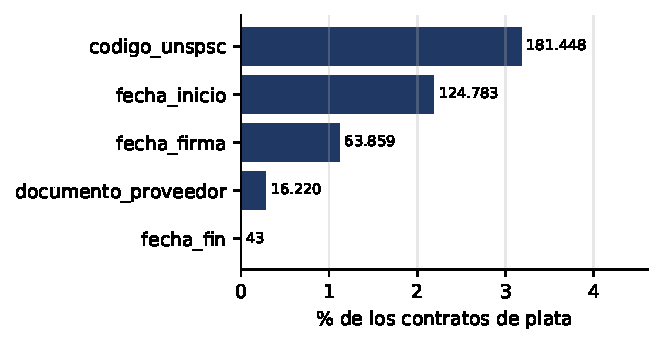
\includegraphics[width=\columnwidth]{fig_nulos.pdf}
\caption{Columnas de plata con nulos (porcentaje del total; etiqueta: número de contratos).}
\label{fig:nulos}
\end{figure}

El nulo en \code{documento\_proveedor} es informativo: un contrato público sin un documento válido del
contratista no permite saber a quién se le pagó, y por eso es una de las nueve alertas. Además, 43.668 contratos
valen cero (comodatos y acuerdos marco, en su mayoría, donde es legítimo) y 644 terminan antes de empezar; para
estos últimos el plazo es negativo y la regla de adiciones exige un plazo positivo. El corte del 11 de noviembre
tenía 67.098 firmas nulas; las cargas diarias completan fechas que la API publica con retraso.

\subsection{Valores extremos}
\label{sec:outliers}
El valor del contrato tiene una cola derecha extrema: en la muestra, la asimetría del valor es 60,7 y la de
$\log_{10}$(valor) es 0,24 (Fig.~\ref{fig:hist}). Por eso el análisis usa la escala logarítmica, y se aplican
dos reglas con fines distintos.

\textbf{1. Regla de calidad (valor no confiable).} Un contrato individual de más de 1~billón de pesos
($10^{12}$~COP) casi siempre es un error de digitación: el máximo es $4{,}4\times10^{17}$~COP, cientos de veces el
presupuesto anual de la nación. Esos \textbf{85 contratos} se conservan con \code{valor\_confiable = false} para
revisarlos aparte, y sus valores no se suman en ninguna tabla de oro. Con esa regla, el valor confiable con
fecha de firma es de 861,1~billones de pesos.

\textbf{2. Regla estadística (valor atípico).} Siguiendo el criterio de Tukey~\cite{tukey} con el factor de
valores ``lejanos'', un contrato es atípico si su valor supera $Q_3+3\,\mathrm{IQR}$ \emph{de su mismo tipo de
contrato}; una obra y una prestación de servicios no se comparan entre sí. Glue (Spark) marca
\textbf{237.446 contratos} (4,16~\%); Athena, con otro algoritmo de cuantiles aproximados, cuenta 236.680
(diferencia del 0,3~\%). La Tabla~\ref{tab:outliers} y la Fig.~\ref{fig:box} muestran los umbrales de los tipos
más frecuentes. El contrato atípico no se elimina: es la alerta de valor atípico.

\begin{table}[t]
\centering
\caption{Regla $Q_3+3\,\mathrm{IQR}$ por tipo de contrato (millones de COP; toda la tabla, en Athena)}
\label{tab:outliers}
\footnotesize
\begin{tabular}{@{}lrrrr@{}}
\toprule
Tipo & Contratos & Mediana & Umbral & Atípicos \\
\midrule
Prest. de servicios & 4.894.743 & 18,7 & 113,7 & 155.564 \\
Otro & 205.545 & 143,2 & 2.404,0 & 17.135 \\
Decreto 092 de 2017 & 204.340 & 15,1 & 184,2 & 24.356 \\
Suministros & 137.738 & 37,6 & 394,0 & 13.613 \\
Compraventa & 111.031 & 28,3 & 317,3 & 11.442 \\
Obra & 50.397 & 216,8 & 3.375,6 & 5.403 \\
\bottomrule
\end{tabular}
\end{table}

\begin{figure}[t]
\centering
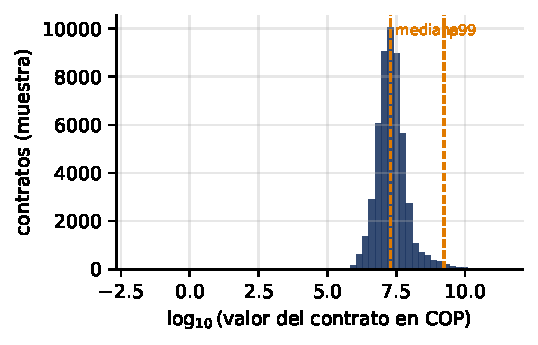
\includegraphics[width=\columnwidth]{fig_hist_valor.pdf}
\caption{Distribución de $\log_{10}$ del valor (muestra de 51.570 contratos, solo valores confiables y
positivos).}
\label{fig:hist}
\end{figure}

\begin{figure}[t]
\centering
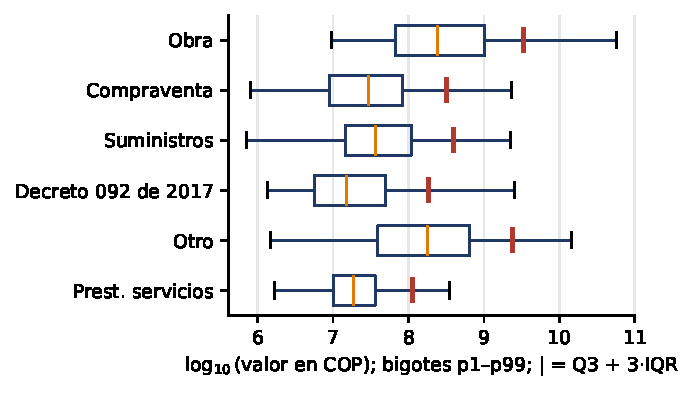
\includegraphics[width=\columnwidth]{fig_box_tipo.pdf}
\caption{Valor por tipo de contrato (muestra). La marca roja es el umbral $Q_3+3\,\mathrm{IQR}$ calculado sobre
toda la tabla.}
\label{fig:box}
\end{figure}

\subsection{Análisis exploratorio}
\label{sec:eda}
El EDA combina agregados exactos de oro (series y conteos) con una muestra determinista de \textbf{51.570
contratos} (0,9~\%), elegida con un \emph{hash} del identificador: la misma consulta devuelve siempre la misma
muestra, sin sesgo por fecha ni por entidad.

\textbf{Modalidad.} La contratación directa reúne el 76,6~\% de los contratos y el 32,2~\% del valor
(Fig.~\ref{fig:modalidades}); le siguen el régimen especial (13,2~\%) y la mínima cuantía (5,5~\%). Son muchos
contratos pequeños, sobre todo de prestación de servicios: este tipo tiene el 85,8~\% de los contratos y una
mediana de 18,7~millones de pesos.

\begin{figure}[t]
\centering
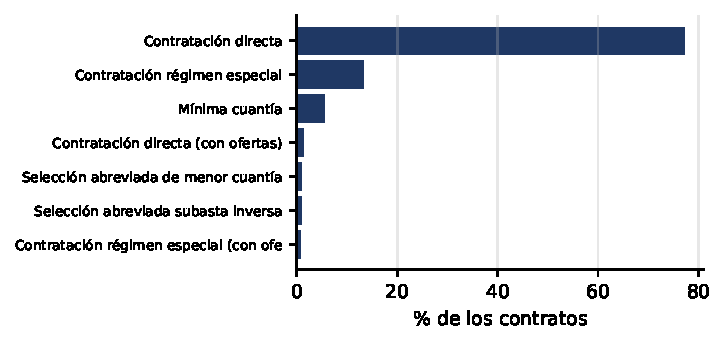
\includegraphics[width=\columnwidth]{fig_modalidades.pdf}
\caption{Contratos por modalidad de contratación (las siete más frecuentes).}
\label{fig:modalidades}
\end{figure}

\textbf{Territorio.} Bogotá concentra 1,85 millones de contratos (32,9~\%), seguida de Valle del Cauca y
Antioquia (Fig.~\ref{fig:departamentos}). El porcentaje de contratación directa varía entre departamentos: 75,7~\%
en Bogotá y 90,1~\% en Valle del Cauca.

\begin{figure}[t]
\centering
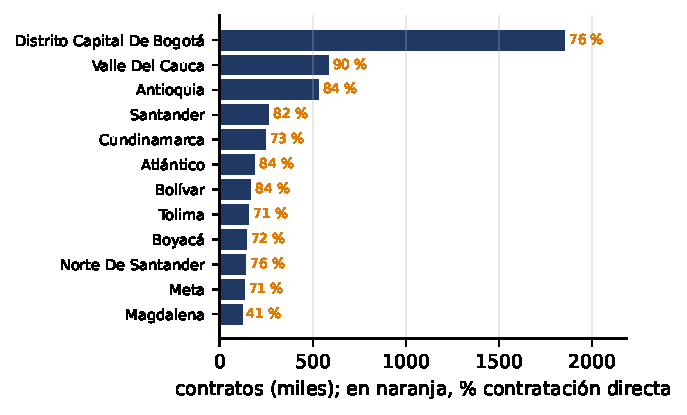
\includegraphics[width=\columnwidth]{fig_departamentos.pdf}
\caption{Los 12 departamentos con más contratos y su porcentaje de contratación directa.}
\label{fig:departamentos}
\end{figure}

\textbf{Estacionalidad y Ley de Garantías.} Contra la hipótesis inicial de un pico en diciembre, el mes con más
contratos de cada año es enero o febrero (Fig.~\ref{fig:serie}): las entidades contratan al inicio de la
vigencia fiscal, sobre todo prestación de servicios. Los picos más altos son enero de 2022 (294.128) y enero de
2026 (487.354), justo antes de las restricciones de la Ley de Garantías por las elecciones presidenciales. En
esos años el porcentaje de contratación directa cae de más del 80~\% a menos del 20~\% durante la restricción. En
2026, según el informe del proyecto (corte del 11 de noviembre), los contratos directos no exceptuados pasaron de
422.012 en el mes previo a 4.690 en toda la restricción. Antes de 2020 el volumen mensual es bajo, lo que
probablemente refleja la adopción gradual de SECOP~II.

\begin{figure*}[t]
\centering
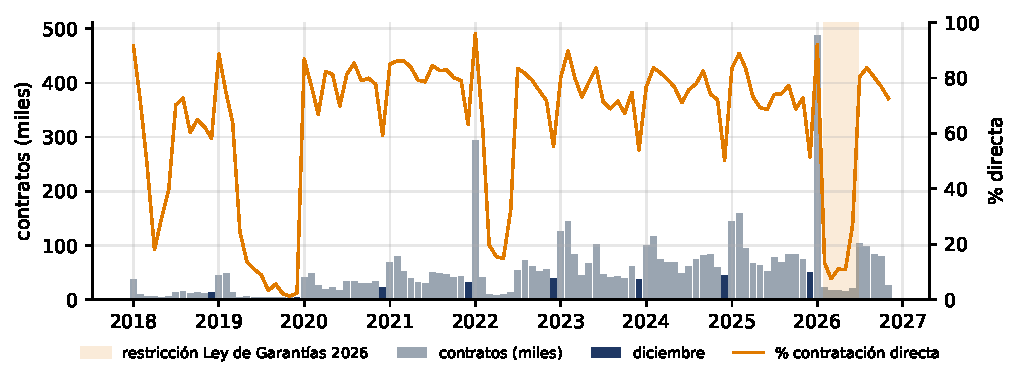
\includegraphics[width=0.9\textwidth]{fig_serie_mensual.pdf}
\caption{Contratos por mes (barras; diciembre resaltado) y porcentaje de contratación directa (línea),
2018--2026. La franja naranja es la restricción de la Ley de Garantías de 2026 (31 de enero al 21 de junio).}
\label{fig:serie}
\end{figure*}

\textbf{Día de firma y plazo.} En la muestra, el 5,8~\% de los contratos se firmó en sábado o domingo, y el
plazo pactado tiene una mediana de 152 días, con picos en múltiplos de mes y en un año
(Fig.~\ref{fig:diaplazo}).

\begin{figure*}[t]
\centering
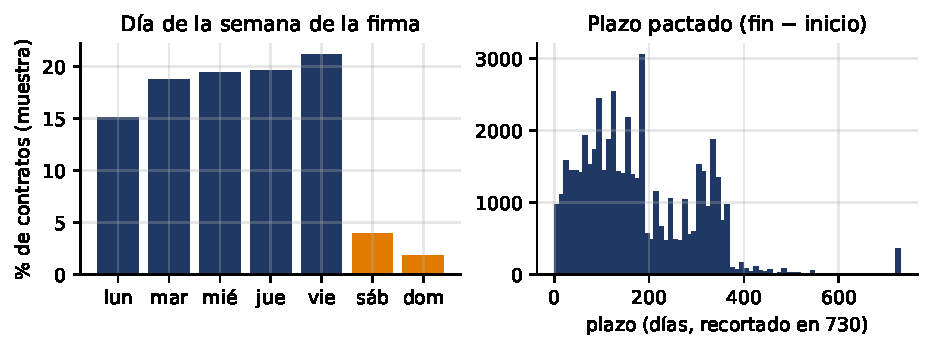
\includegraphics[width=0.9\textwidth]{fig_dia_plazo.pdf}
\caption{Día de la semana de la firma (fin de semana en naranja) y plazo pactado (muestra de 51.570 contratos).}
\label{fig:diaplazo}
\end{figure*}

\textbf{Alertas.} El 83,6~\% de los contratos (4.769.925) tiene al menos una alerta, sobre todo por la
contratación directa (Fig.~\ref{fig:alertas}). Sin ella, las alertas son raras: fin de semana 5,8~\%, valor
atípico 4,2~\%, inicio antes de la firma 3,7~\%, y anticipo mayor al 50~\% solo en 162 contratos. Esto obliga a
mirar perfiles y combinaciones, no conteos sueltos, y motiva las dos técnicas siguientes.

\begin{figure}[t]
\centering
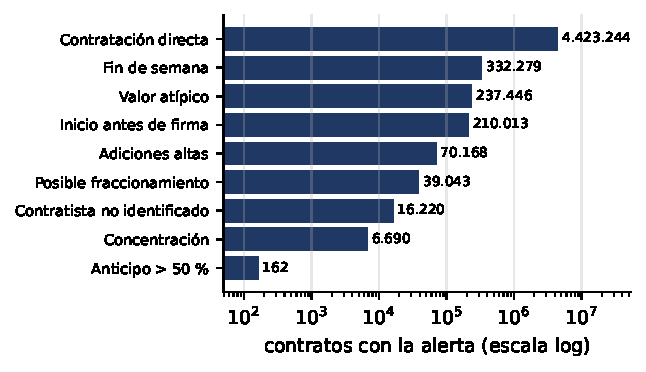
\includegraphics[width=\columnwidth]{fig_frecuencia_alertas.pdf}
\caption{Contratos con cada alerta (todos los contratos de oro, escala logarítmica).}
\label{fig:alertas}
\end{figure}

\subsection{Agrupamiento de entidades con K-means}
\label{sec:kmeans}
\textbf{Datos.} La tabla \code{gold\_riesgo\_entidades} tiene 5.121 entidades (por NIT). Se toman las 2.604 con
al menos 20 contratos, el mismo mínimo del ranking, porque con menos contratos los porcentajes son inestables; se
descarta una sin ningún valor confiable, y quedan \textbf{2.603 entidades} con el 99,8~\% de los contratos.

\textbf{Variables.} Ocho por entidad: el porcentaje de sus contratos con siete alertas (directa, fin de semana,
inicio antes de la firma, valor atípico, fraccionamiento, adiciones altas y contratista no identificado) y la
participación del mayor contratista en su valor. Se excluyen el anticipo alto, que solo aparece en el 1,6~\% de
las entidades y casi no tiene varianza, y el porcentaje de la alerta de concentración, que repite la
participación del mayor contratista. Las correlaciones de Spearman entre variables son bajas o moderadas
(Fig.~\ref{fig:corr}), así que ninguna es redundante.

\textbf{Preprocesamiento.} A cada proporción $p$ se le aplica $\sqrt{p}$, que estabiliza la varianza de
porcentajes con muchos ceros y colas largas, y luego se estandariza (media 0, desviación 1) para que ninguna
variable domine la distancia euclidiana.

\begin{figure}[t]
\centering
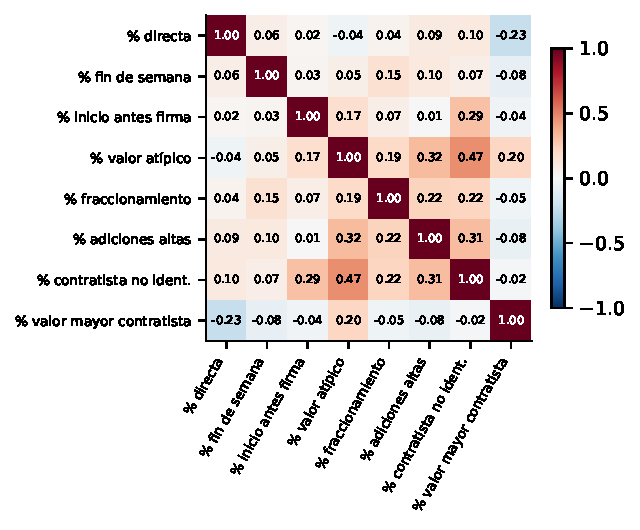
\includegraphics[width=0.92\columnwidth]{fig_correlacion_entidades.pdf}
\caption{Correlación de Spearman entre las variables de las 2.603 entidades.}
\label{fig:corr}
\end{figure}

\textbf{Modelo y elección de $k$.} K-means~\cite{macqueen} con inicialización k-means++~\cite{kmeanspp}
(scikit-learn~\cite{sklearn}), 20 inicios por $k$ y semilla 42. Se evaluó $k=2,\dots,10$ con la inercia
(método del codo), el coeficiente de silhouette~\cite{silhouette} y el índice de Davies-Bouldin~\cite{davies}
(Fig.~\ref{fig:codo}). La inercia baja sin un codo marcado; la silhouette es máxima en $k=4$ (0,213) entre
$k\geq3$ y cae a partir de $k=7$. Se descartó $k=2$ (0,207) porque solo separa ``mucha o poca contratación
directa'', algo poco útil para priorizar. El modelo final ($k=4$, 50 inicios) tiene silhouette de 0,213 y
Davies-Bouldin de 1,73.

\begin{figure*}[t]
\centering
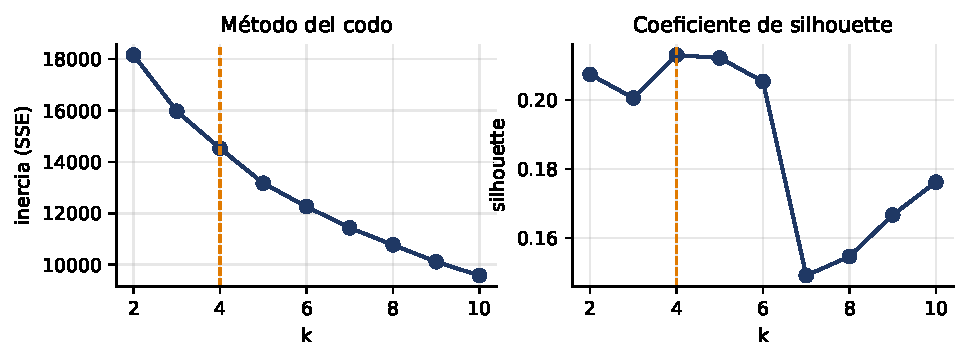
\includegraphics[width=0.9\textwidth]{fig_codo_silhouette.pdf}
\caption{Selección de $k$: inercia (método del codo) y coeficiente de silhouette. La línea naranja marca $k=4$.}
\label{fig:codo}
\end{figure*}

\textbf{Estabilidad.} Al repetir K-means con 10 semillas distintas, el índice de Rand ajustado~\cite{ari}
frente al modelo final es de 0,999 en promedio (mínimo 0,998): los grupos no dependen del azar de la
inicialización. Una silhouette de 0,21 indica, eso sí, que los grupos se traslapan: son perfiles, no categorías
separadas (Fig.~\ref{fig:pca}; las dos primeras componentes principales explican el 37,8~\% de la varianza).

\begin{figure}[t]
\centering
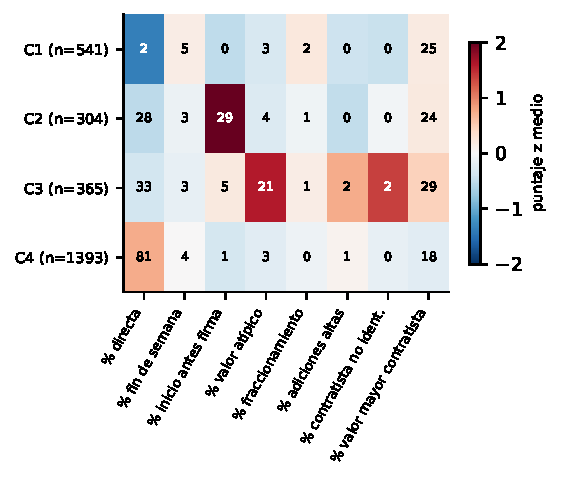
\includegraphics[width=\columnwidth]{fig_perfil_clusters.pdf}
\caption{Perfil de los clústeres: el color es el puntaje $z$ medio y el número es el porcentaje medio de cada
variable.}
\label{fig:perfil}
\end{figure}

\begin{figure}[t]
\centering
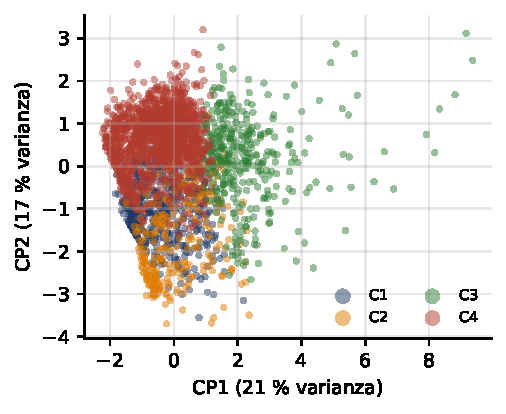
\includegraphics[width=0.9\columnwidth]{fig_pca_clusters.pdf}
\caption{Entidades proyectadas en las dos primeras componentes principales, coloreadas por clúster.}
\label{fig:pca}
\end{figure}

\textbf{Interpretación} (Fig.~\ref{fig:perfil}, Tabla~\ref{tab:clusters}):
\begin{itemize}
  \item \textbf{C1, alertas bajas (541 entidades).} Solo el 13,5~\% de sus contratos tiene alguna alerta y casi
        no usa contratación directa. Abundan las empresas sociales del Estado (hospitales), que contratan por
        régimen especial; por eso una directa baja no equivale siempre a más competencia.
  \item \textbf{C2, inicio antes de la firma (304).} En promedio, el 29~\% de sus contratos empezó a ejecutarse
        antes de firmarse, ocho veces la media nacional (3,7~\%).
  \item \textbf{C3, valores atípicos (365).} El 21~\% de sus contratos supera el umbral de su tipo, y tiene los
        porcentajes más altos de adiciones altas (2,4~\%), contratista no identificado (2,1~\%) y participación
        del mayor contratista (29~\%).
  \item \textbf{C4, contratación directa predominante (1.393).} La mitad de las entidades y el 77,8~\% de los
        contratos. El 80,6~\% de sus contratos es directo; las demás alertas están cerca de la media.
\end{itemize}

\begin{table}[t]
\centering
\caption{Resumen de los clústeres (medias por entidad)}
\label{tab:clusters}
\footnotesize
\begin{tabular}{@{}lrrrr@{}}
\toprule
 & C1 & C2 & C3 & C4 \\
\midrule
Entidades & 541 & 304 & 365 & 1.393 \\
Contratos (miles) & 381,5 & 292,3 & 590,4 & 4.426,5 \\
Mediana de contratos & 148 & 186 & 435 & 625 \\
\% con alguna alerta & 13,5 & 55,8 & 58,9 & 83,7 \\
\% directa & 1,6 & 28,3 & 33,2 & 80,6 \\
\% inicio antes de firma & 0,3 & 29,0 & 4,8 & 0,8 \\
\% valor atípico & 3,1 & 3,5 & 21,1 & 2,6 \\
\% mayor contratista & 24,6 & 24,3 & 29,3 & 17,8 \\
\bottomrule
\end{tabular}
\end{table}

Así, el índice de un solo número del objetivo~2 se complementa con un \emph{tipo} de patrón: a una entidad de C2
conviene revisarle las fechas de ejecución, y a una de C3, los valores y las adiciones.

\subsection{Reglas de asociación entre alertas}
\label{sec:apriori}
\textbf{Planteamiento.} Cada contrato es una transacción y cada alerta activa es un ítem. En lugar de descargar
5,7 millones de filas, Athena agrupa los contratos por su combinación de las nueve alertas: salen 129
combinaciones distintas con su número de contratos. Con esa tabla, el soporte de cualquier conjunto de alertas
se calcula \textbf{exacto} sobre todos los contratos.

\textbf{Algoritmo.} Apriori~\cite{apriori}, implementado en el proyecto: genera los conjuntos frecuentes nivel por
nivel y descarta un candidato si alguno de sus subconjuntos no es frecuente. Con soporte mínimo de 0,1~\%
(unos 5.700 contratos) se evaluaron 47 candidatos y salieron 21 conjuntos frecuentes y 30 reglas. Para cada regla
$A\Rightarrow B$:
\begin{equation}
\mathrm{conf}=\frac{\mathrm{sop}(A\cup B)}{\mathrm{sop}(A)},\qquad
\mathrm{lift}=\frac{\mathrm{conf}}{\mathrm{sop}(B)} .
\end{equation}
Un lift mayor que 1 indica que las alertas aparecen juntas más de lo esperado si fueran independientes.

\begin{table}[t]
\centering
\caption{Reglas con lift $\geq1{,}2$ (soporte mínimo 0,1~\%; todos los contratos)}
\label{tab:reglas}
\footnotesize
\begin{tabular}{@{}L{3.6cm}rrr@{}}
\toprule
Regla & Contratos & Conf. & Lift \\
\midrule
no identificado $\Rightarrow$ valor atípico & 7.170 & 44,2~\% & 10,62 \\
adiciones altas $\Rightarrow$ fin de semana & 9.846 & 14,0~\% & 2,41 \\
adiciones altas $\Rightarrow$ inicio antes de firma & 6.089 & 8,7~\% & 2,36 \\
adiciones altas $\Rightarrow$ valor atípico & 6.251 & 8,9~\% & 2,14 \\
inicio antes de firma $\Rightarrow$ valor atípico & 11.687 & 5,6~\% & 1,34 \\
\midrule
\multicolumn{4}{@{}l}{\emph{Asociaciones negativas (lift $<1$):}} \\
valor atípico $\Rightarrow$ directa & 105.150 & 44,3~\% & 0,57 \\
adiciones altas $\Rightarrow$ directa & 17.161 & 24,5~\% & 0,32 \\
\bottomrule
\end{tabular}
\end{table}

\begin{figure}[t]
\centering
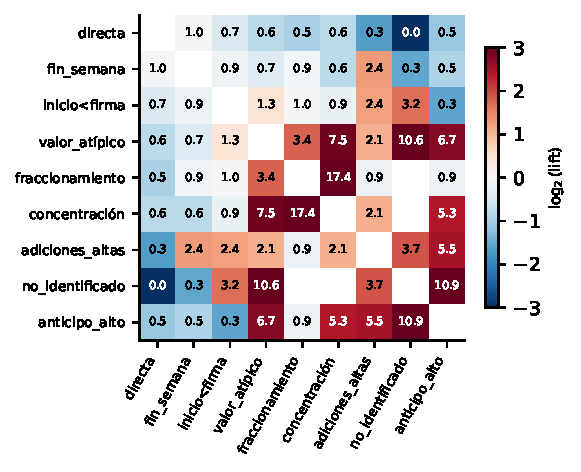
\includegraphics[width=0.92\columnwidth]{fig_lift_pares.pdf}
\caption{Lift entre pares de alertas (todos los pares, incluso bajo el soporte mínimo). Rojo: aparecen juntas
más de lo esperado; azul: menos. Las celdas vacías son pares que no coinciden en ningún contrato.}
\label{fig:lift}
\end{figure}

\textbf{Resultados} (Tabla~\ref{tab:reglas}, Fig.~\ref{fig:lift}):
\begin{itemize}
  \item La regla más fuerte es \emph{contratista no identificado $\Rightarrow$ valor atípico}: el 44,2~\% de los
        contratos sin documento del contratista tiene un valor atípico, 10,6 veces lo esperado. Es la única regla
        con confianza superior al 30~\%, y apunta tanto a contratos para revisar como a un problema de calidad en
        la publicación.
  \item Las adiciones altas se asocian con firmar en fin de semana, con iniciar antes de la firma y con valores
        atípicos (lift de 2,1 a 2,4): contratos con problemas de planeación tienden a acumular varias alertas.
  \item Bajo el soporte mínimo aparecen asociaciones aún más altas, como fraccionamiento con concentración (lift
        17,4), útiles para casos puntuales.
  \item La contratación directa se asocia de forma \emph{negativa} con casi todas las demás alertas (lift entre
        0,05 y 0,97): son, en su mayoría, contratos pequeños de servicios con fechas y valores habituales. Por
        eso la directa sola no debe dominar el índice, y conviene ponderar las alertas.
  \item Algunos pares son imposibles por construcción (contratista no identificado con fraccionamiento o
        concentración, que exigen un documento) y no son hallazgos.
\end{itemize}

\subsection{Reproducibilidad}
Todo el módulo está en la carpeta \code{mineria/} del repositorio: \code{sql/} (nueve consultas de Athena),
\code{01\_extraer\_athena.py} (las ejecuta con el AWS CLI y deja una bitácora con el identificador de cada
consulta y los bytes escaneados), \code{02\_eda.py}, \code{03\_clustering\_kmeans.py} y
\code{04\_reglas\_asociacion.py}. Usan pandas, NumPy, Matplotlib y scikit-learn, con semilla fija; la muestra
es determinista. Las nueve consultas escanearon 237~MB en total: con la tarifa de Athena de 5~USD por TB
escaneado~\cite{athenapricing}, menos de un centavo de dólar. En el computador local solo se procesan unas
57.000 filas.

% =============================================================================
\section{Discusión y limitaciones}
% =============================================================================
\begin{itemize}
  \item Las alertas y los clústeres describen \emph{patrones}, no conductas. Un inicio antes de la firma puede
        deberse a un error de registro; un valor atípico, a un contrato grande legítimo.
  \item La silhouette de 0,21 muestra grupos traslapados. Los clústeres sirven para orientar la revisión, no como
        una clasificación definitiva.
  \item Las entidades nacionales con un solo NIT y muchas sedes (por ejemplo, regionales de una misma entidad)
        quedan agregadas con un nombre y un departamento únicos, y esto distorsiona el análisis territorial.
  \item Los contratos sin código UNSPSC se agrupan juntos en la regla de fraccionamiento, lo que puede inflar esa
        alerta en entidades que no publican el código.
  \item Las cifras cambian cada día con la carga diaria; este informe usa el corte del 13 de noviembre de 2026.
\end{itemize}

% =============================================================================
\section{Conclusiones y trabajo futuro}
% =============================================================================
El trabajo se propuso facilitar a la ciudadanía y a los entes de control la vigilancia de la contratación pública. El objetivo se cumplió: plata es un conjunto limpio de 5.702.270 contratos sin duplicados, con nulos documentados y tratados sin
imputación, y con dos reglas de valores extremos: una de calidad (85 contratos) y otra estadística (237.446). El
EDA corrigió una hipótesis (el pico es en enero o febrero, no en diciembre) y mostró el efecto de la Ley de
Garantías en la contratación directa. K-means separó cuatro perfiles de entidades estables y fáciles de
interpretar, y Apriori, con soporte exacto sobre todos los contratos, mostró qué alertas se refuerzan entre sí.

Para el informe final se propone: ponderar las alertas en el índice según su rareza y sus asociaciones; probar
métodos robustos a grupos traslapados (por ejemplo, DBSCAN o mezclas gaussianas); validar una muestra de casos con
revisión manual; redactar el documento completo en inglés; y, como trabajo futuro, orquestar un equipo de agentes de inteligencia artificial que lea los documentos de cada contrato (PDF u otros formatos publicados en SECOP~II) y analice anomalías que no se ven en los datos tabulares, como diferencias entre el objeto, el valor, los plazos y los anexos del contrato.

% -----------------------------------------------------------------------------
\begin{thebibliography}{99}
\bibitem{secop} Agencia Nacional de Contratación Pública -- Colombia Compra Eficiente, ``SECOP II -- Contratos Electrónicos,'' Portal de Datos Abiertos de Colombia, conjunto \texttt{jbjy-vk9h}, 2026. [En línea]. Disponible: \url{https://www.datos.gov.co/d/jbjy-vk9h}
\bibitem{medallion} Databricks, ``What is the medallion lakehouse architecture?,'' documentación, 2026. [En línea]. Disponible: \url{https://docs.databricks.com/aws/en/lakehouse/medallion}
\bibitem{lakehouse} M. Armbrust, A. Ghodsi, R. Xin y M. Zaharia, ``Lakehouse: A new generation of open platforms that unify data warehousing and advanced analytics,'' en \emph{Proc. Conf. Innovative Data Systems Research (CIDR)}, 2021.
\bibitem{ocp} Open Contracting Partnership, ``Red flags for integrity: Giving the green light to open data solutions,'' 2016. [En línea]. Disponible: \url{https://www.open-contracting.org/resources/red-flags-integrity-giving-green-light-open-data-solutions/}
\bibitem{fazekas} M. Fazekas y G. Kocsis, ``Uncovering high-level corruption: Cross-national objective corruption risk indicators using public procurement data,'' \emph{British J. Political Science}, vol.~50, n.º~1, pp.~155--164, 2020.
\bibitem{ley996} Congreso de la República de Colombia, ``Ley 996 de 2005 (Ley de Garantías Electorales),'' art.~33, \emph{Diario Oficial} n.º~46.102, 24 nov. 2005.
\bibitem{ley80} Congreso de la República de Colombia, ``Ley 80 de 1993, Estatuto General de Contratación de la Administración Pública,'' art.~40, \emph{Diario Oficial} n.º~41.094, 28 oct. 1993.
\bibitem{ods16} Naciones Unidas, ``Objetivo 16: Promover sociedades justas, pacíficas e inclusivas,'' Objetivos de Desarrollo Sostenible, 2026. [En línea]. Disponible: \url{https://www.un.org/sustainabledevelopment/es/peace-justice/}
\bibitem{ley1712} Congreso de la República de Colombia, ``Ley 1712 de 2014, por medio de la cual se crea la Ley de Transparencia y del Derecho de Acceso a la Información Pública Nacional,'' \emph{Diario Oficial} n.º~49.084, 6 mar. 2014.
\bibitem{soda} Tyler Technologies, ``Socrata Open Data API (SODA) documentation,'' 2026. [En línea]. Disponible: \url{https://dev.socrata.com/}
\bibitem{spark} M. Zaharia \emph{et al.}, ``Apache Spark: A unified engine for big data processing,'' \emph{Commun. ACM}, vol.~59, n.º~11, pp.~56--65, 2016, doi: 10.1145/2934664.
\bibitem{iceberg} The Apache Software Foundation, ``Apache Iceberg table format specification,'' 2026. [En línea]. Disponible: \url{https://iceberg.apache.org/spec/}
\bibitem{tukey} J. W. Tukey, \emph{Exploratory Data Analysis}. Reading, MA, EE.~UU.: Addison-Wesley, 1977.
\bibitem{macqueen} J. MacQueen, ``Some methods for classification and analysis of multivariate observations,'' en \emph{Proc. 5th Berkeley Symp. Mathematical Statistics and Probability}, vol.~1, 1967, pp.~281--297.
\bibitem{kmeanspp} D. Arthur y S. Vassilvitskii, ``k-means++: The advantages of careful seeding,'' en \emph{Proc. 18th Annu. ACM-SIAM Symp. Discrete Algorithms (SODA)}, 2007, pp.~1027--1035.
\bibitem{sklearn} F. Pedregosa \emph{et al.}, ``Scikit-learn: Machine learning in Python,'' \emph{J. Machine Learning Research}, vol.~12, pp.~2825--2830, 2011.
\bibitem{silhouette} P. J. Rousseeuw, ``Silhouettes: A graphical aid to the interpretation and validation of cluster analysis,'' \emph{J. Computational and Applied Mathematics}, vol.~20, pp.~53--65, 1987.
\bibitem{davies} D. L. Davies y D. W. Bouldin, ``A cluster separation measure,'' \emph{IEEE Trans. Pattern Anal. Mach. Intell.}, vol.~PAMI-1, n.º~2, pp.~224--227, 1979.
\bibitem{ari} L. Hubert y P. Arabie, ``Comparing partitions,'' \emph{J. Classification}, vol.~2, n.º~1, pp.~193--218, 1985.
\bibitem{apriori} R. Agrawal y R. Srikant, ``Fast algorithms for mining association rules,'' en \emph{Proc. 20th Int. Conf. Very Large Data Bases (VLDB)}, 1994, pp.~487--499.
\bibitem{athenapricing} Amazon Web Services, ``Amazon Athena pricing,'' 2026. [En línea]. Disponible: \url{https://aws.amazon.com/athena/pricing/}
\end{thebibliography}

\end{document}
